% a mashup of hipstercv, friggeri and twenty cv
% https://www.latextemplates.com/template/twenty-seconds-resumecv
% https://www.latextemplates.com/template/friggeri-resume-cv

\documentclass[lighthipster]{simplehipstercv}
% available options are: darkhipster, lighthipster, pastel, allblack, grey, verylight, withoutsidebar
% withoutsidebar
\usepackage[utf8]{inputenc}
\usepackage[default]{raleway}
\usepackage[margin=1cm, a4paper]{geometry}
\usepackage{hyperref}
%\usepackage[UTF8]{ctex}
\hypersetup{hidelinks}


%------------------------------------------------------------------ Variablen

\newlength{\rightcolwidth}
\newlength{\leftcolwidth}
\setlength{\leftcolwidth}{0.23\textwidth}
\setlength{\rightcolwidth}{0.75\textwidth}

%------------------------------------------------------------------
\title{New Simple CV}
\author{\LaTeX{} Ninja}
\date{June 2019}

\pagestyle{empty}
\begin{document}


\thispagestyle{empty}
%-------------------------------------------------------------

\section*{Start}

\simpleheader{headercolour}{Shuang}{Song}{Ph.D. candidate in Physical Geography, Beijing Normal University, China.}{white}



%------------------------------------------------

% this has to be here so the paracols starts..
\subsection*{}
\vspace{3em}

\setlength{\columnsep}{1.5cm}
\columnratio{0.23}[0.75]
\begin{paracol}{2}
\hbadness5000
%\backgroundcolor{c[1]}[rgb]{1,1,0.8} % cream yellow for column-1 %\backgroundcolor{g}[rgb]{0.8,1,1} % \backgroundcolor{l}[rgb]{0,0,0.7} % dark blue for left margin

\paracolbackgroundoptions

% 0.9,0.9,0.9 -- 0.8,0.8,0.8


\footnotesize
{\setasidefontcolour
\flushright
% \begin{center}
\begin{figure}
    \centering
    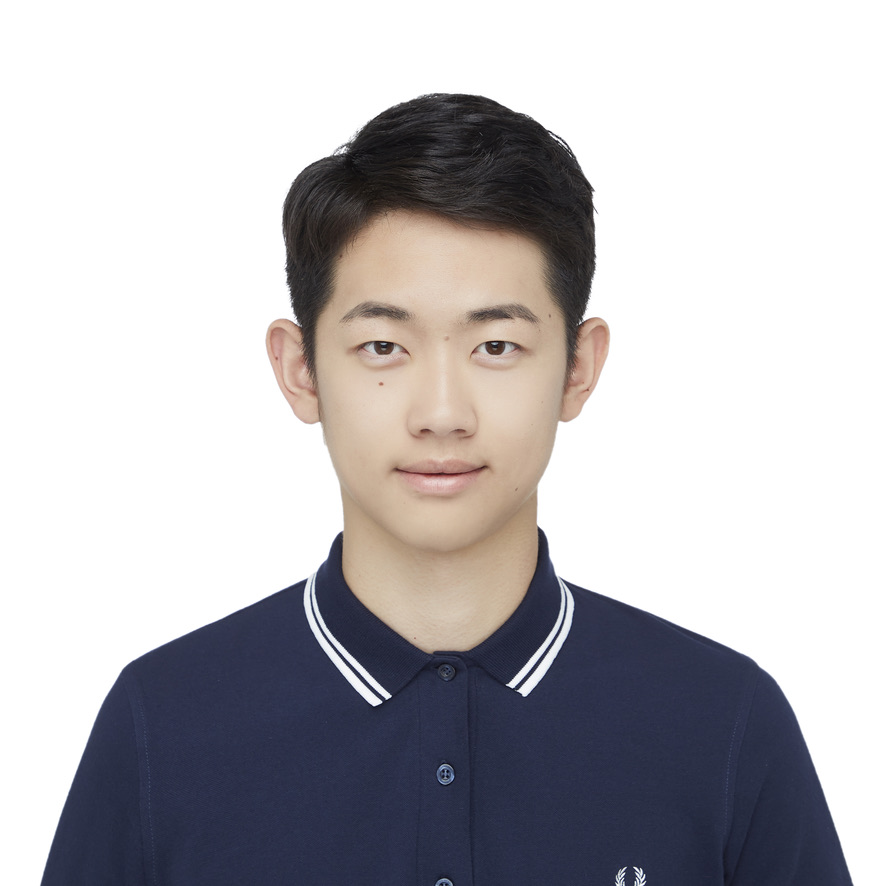
\includegraphics[width=0.2\textwidth]{shuangsong.jpeg}
\end{figure}
% \roundpic{shuangsong.jpeg}
% \end{center}

\bg{cvgreen}{white}{Basic information}\\[0.5em]
% \textbf{Shuang Song} is a PhD candidate in geography, focusing on human-water relationships and complex system modelling. At the same time, he is also a traveller and a writer. Through my research and writing, I hope to call attention to our relationship with nature. \& space.}
\textbf{Name}: Shuang Song

\textbf{Birth}: December 24th 1996

\textbf{Nationality}: China

\textbf{Institution}: Beijing Normal University
\bigskip

\bg{cvgreen}{white}{\faMapMarker{ } Address} \\[0.5em]

No.19, Xinjiekouwai St. Haidian District, Beijing, China, 100875

\bigskip

% \bg{cvgreen}{white}{Areas of specialization} \\[0.5em]

% Privateering ~•~ Bucaneering ~•~ Parler ~•~ Rum

% \bigskip



% \bigskip
\bg{cvred}{white}{\faUniversity{ } Research Experiences}\\[0.5em]

\texttt{Water Resources Management}

\texttt{Human-water relationship}

\texttt{Social-ecological systems}

\texttt{Complex system modelling}

\texttt{Integrated geography}

\texttt{Socio-hydrology}

\bigskip
\begin{minipage}[t]{0.2\textwidth}
    \section*{Programming}
    \begin{tabular}{r @{\hspace{0.5em}}l}
         \bg{skilllabelcolour}{iconcolour}{Python} &  \barrule{0.55}{0.5em}{cvred}\\
         \bg{skilllabelcolour}{iconcolour}{Shell} & \barrule{0.50}{0.5em}{cvred} \\
         \bg{skilllabelcolour}{iconcolour}{\LaTeX} & \barrule{0.50}{0.5em}{cvgreen} \\
		 \bg{skilllabelcolour}{iconcolour}{R} & \barrule{0.3}{0.5em}{cvgreen} \\
         \bg{skilllabelcolour}{iconcolour}{MatLab} & \barrule{0.2}{0.5em}{cvgreen} \\     
        %  \bg{skilllabelcolour}{iconcolour}{javascript} & \barrule{0.1}{0.5em}{cvpurple} \\
    \end{tabular}
\end{minipage}

\bigskip
\begin{minipage}[t]{0.2\textwidth}
    \section*{Languages}
    \begin{tabular}{l | l}
    \textbf{Chinese} & {\phantom{x}\footnotesize mother tongue} \\
    \textbf{English} & \pictofraction{\faCircle}{cvgreen}{4}{black!30}{1}{\tiny} \\
    % \textbf{Spanish} & \pictofraction{\faCircle}{cvgreen}{1}{black!30}{4}{\tiny} \\
    % \textbf{Italian} & \pictofraction{\faCircle}{cvgreen}{3}{black!30}{2}{\tiny}
    \end{tabular}
\end{minipage}
\bigskip

\vspace{4em}

\infobubble{\faAt}{cvgreen}{white}{\href{www.SongshGeo.com}{SongshGeo.com}}
\infobubble{\faTwitter}{cvgreen}{white}{\href{https://twitter.com/ShuangSong11}{@ShuangSong11}}
% \infobubble{\faFacebook}{cvgreen}{white}{Shuang Song}
\infobubble{\faGithub}{cvgreen}{white}{\href{https://github.com/SongshGeo}{SongshGeo}}

\phantom{turn the page}

\phantom{turn the page}
}
%-----------------------------------------------------------
\switchcolumn

\small
\section*{Research Descriptions}
Mr. Shuang Song is a Ph.D. candidate at the State Key Laboratory of Earth Surface Processes and Resource Ecology, Beijing Normal University. His ongoing Ph.D. projects include quantitative analyses of human activities' impact on water resources and socio-hydrological systems modeling. His work also includes integrated geography and landscape ecology.

\section*{Educational Experiences}

\begin{tabular}{r| p{0.6\textwidth} c}
    \cvevent{2018--now}{Ph.D. Candidate in Geography}{Beijing Normal University}{Beijing, China \color{cvred}}{
	    \textbf{Representative Courses:} Agent-based modelling, Complex network analysis, Big data in Geography Analysis, Research Methods of Environmental Evolution, Higher Economic Geography, et al.
    	    
    	\textbf{
    		GPA: 3.7 / 5
    		[Supervisor: \href{https://geot.bnu.edu.cn/Public/htm/news/5/377.html}{Prof. Dr. Shuai Wang} \href{https://geot.bnu.edu.cn/Public/htm/news/5/133.html}{Prof. Dr. Bojie Fu}]}.
    } 
	\vspace{1em}\\
	\newline
	
    \cvevent{2014--2018}{B.S. of Science, Physical Geography \& History Study (The second major)}{Sun Yat-Sen University}{Guangzhou, China \color{cvred}}{
    \textbf{Representative Courses:} Hydrology, Physical Geography, Histrocial Geography. 
    
    \textbf{Dissertation titled:} ``Testing of Human-Flood Model: Taking floodplain of the Yellow River in Ningxia as an exapmle.''
    
    \textbf{
    	GPA: 3.7 / 5
    	[Supervisor: Prof. Dr. Yuxiang Dong]
    }.
    }
\end{tabular}
% \vspace{1em}

\section*{Current Projects \hfill\footnotesize\textbf{\href{https://www.researchgate.net/profile/Shuang-Song-14}{>> more}}}
\begin{tabular}{r| p{0.6\textwidth} c}
	\cvevent{2018-now}{Yellow River Basin's Human-water relationship modelling}{Core Member}{Beijing Normal University \color{cvred}}{
        % 介绍人-水项目
		\textbf{Abstract:} My Ph.D. dissertation titled ``Evolution of human-water relationship and its mechanism in the Yellow River Basin''. Here, I'm working on an Agent-Based Model to emulate the evolution of human-water relationship in the Yellow River Basin, China. 
    } \\

	\cvevent{2017-2020}{Socio-hydrology and sustainability of the Yellow River, China}{Core Member}{Beijing Normal University \color{cvred}}{
		\textbf{Abstract:} Participated in the finished program as a core member. I improved a classical socio-hydrological system dynamics model by coupling a social module. Furthermore, I quantitatively analyzed the regime shift of sediment transport for the past 2000 years in the Yellow River Basin, China, and attributed it to human activities. 
	}
	% \cvevent{2020-now}{Grassland ecological restoration}{Lead}{Beijing Normal University \color{cvred}}{
    %     % 介绍草原生态恢复项目
    %     We perform long-term investigation in Inner Mongolia grassland. We care about how herders' perception and their self-organization management influence the local ecosystem health. 
    % } \\
	% \cvevent{2021-now}{Dream Bottle, a Django-based Web-Software}{Lead}{No founder \color{headerblue}}{
	% 	% 介绍Dream Bottle项目
	% 	I developed an open-resource ``dream bottle'' software for users where they can store and withdraw their wishes in. Have a try through my website \href{www.songshgeo.com}{songshgeo.com}!
	% }
\end{tabular}
%\vspace{1em}

\section*{Academic Publications  \hfill\footnotesize\textbf{\href{https://www.researchgate.net/profile/Shuang-Song-14}{>> more}}}
\begin{tabular}{>{\footnotesize\bfseries}r >{\footnotesize}p{0.6\textwidth} r}
	2021 & \scipubfirst{Decreased Virtual Water Outflows from the Yellow River Basin Are Increasingly Critical to China.}{Hydrology and Earth System Science}{5.748}{Q1, openly discussing} \\
    2021 & \scipubfirst{Improving representation of collective memory in socio‐hydrological models and new insights into flood risk management.}{Journal of Flood Risk Management}{3.884}{Q2} \\
    2021 & \scipubfirst{The responses of \textit{Spinifex littoreus} to sand burial on the coastal area of Pingtan Island, Fujian Province, South China.}{Écoscience}{1.950}{Q4} \\
    2020 & \scipubsecond{Shuai Wang}{Achieving a Fit between Social and Ecological Systems in Drylands for Sustainability}{Current Opinion in Environmental Sustainability}{6.984}{Q2} \\
	2020 & \scipubfirst{Sediment transport under increasing anthropogenic stress: Regime shifts within the Yellow River, China.}{Ambio}{5.129}{Q2} \\
	2019 & \scipubfirst{Study on adaptive governance of social-ecological system: Progress and prospect}{Acta Geographica Sinica}{7.204}{in Chinese} \\
\end{tabular}

\section*{Awards \hfill\footnotesize\textbf{\href{www.songshgeo.com}{}}}
\begin{tabular}{>{\footnotesize\bfseries}r >{\footnotesize}p{0.36\textwidth}r >{\footnotesize}r}
    % \cvdegree{2020}{National Scholarship}{M.A.}{Beijing Normal Univerisy\color{cvred}}{} \\
    \award{2020}{Chinese National Scholarship}{Beijing Normal University}{\color{cvred}} \\
    \award{2019}{Academic Presentation: 1st \& most popular}{Beijing Normal University}{\color{cvred}} \\
    \award{2018}{Excellent Graduation Thesis}{Sun Yat-Sen University}{\color{cvred}}\\
    \award{2017}{Chinese National Scholarship}{Sun Yat-Sen University}{\color{cvred}} \\
    \award{2016}{Chinese National University Geographic Science Presentation: Leader \& 1st \& Most Innovative award.}{Geographical Society of China}{\color{cvred}}
    % \award{2020}{}
\end{tabular}


% \section*{Public Presentation \hfill\footnotesize\textbf{\href{www.songshgeo.com}{>> more}}}
% \begin{tabular}{>{\footnotesize\bfseries}r >{\footnotesize}p{0.4\textwidth}r  >{\footnotesize}p{0.12\textwidth}r}
% 	% 2019 & ``Regime shift sediment transport of the Yellow River'', at: \emph{AGU} in San Francisco.
% 	% \pre{2021-10}{Adaptation: the core mechanism of ecosystems}{Invited}{Inner Mongolia}{\color{cvgreen}} \\
%     % \pre{2020-11}{How to do interdisciplinary research: experience sharing}{Invited}{Beijing}{\color{cvgreen}} \\
%     \pre{2019-12}{Regime shift sediment transport of the Yellow River}{AGU}{San Francisco}{\color{cvred}} \\
% \end{tabular}



% \section*{Featured Blog Posts \hfill\footnotesize\textbf{\href{www.songshgeo.com}{>> more}}}
% \begin{tabular}{>{\footnotesize\bfseries}r >{\footnotesize}p{0.3\textwidth} >{\footnotesize}p{0.22\textwidth}l >{\footnotesize}p{0.15\textwidth}r}
%     % 1729 & \emph{test}, Tortuga Printing Press. \\
%     % 1720 & ``Privateering for Beginners'', in: \emph{The Pragmatic Pirate} (1/1720).
%     \blog{2021}{Rivers and lakes: Jiangnan Tour}{\#Travelling, \#Essay}{Wechat}{\color{cvgreen}} \\
%     \blog{2021}{Stop by stop on my journey}{\#Travelling, \#Essay}{Wechat}{\color{cvgreen}} \\
%     \blog{2020}{How to make academic charts}{\#Academic, \#Design}{Wechat}{\color{cvred}} \\
% \end{tabular}


\bigskip
\vfill{} % Whitespace before final footer

%----------------------------------------------------------------------------------------
%	FINAL FOOTER
%----------------------------------------------------------------------------------------
\setlength{\parindent}{0pt}
\begin{minipage}[t]{\rightcolwidth}
\begin{center}\fontfamily{\sfdefault}\selectfont \color{black!70}
{\small \textbf{Shuang Song} \icon{\faEnvelopeO}{cvgreen}{} \href{mailto:SongshGeo@Gmail.com}{SongshGeo@Gmail.com} \icon{\faEnvelopeO}{cvgreen}{} \href{mailto:songshgeo@mail.bnu.edu.cn}{songshgeo@mail.bnu.edu.cn} \newline\icon{\faAt}{cvgreen}{} More information accessible at \href{https://www.researchgate.net/profile/Shuang-Song-14}{Research Gate}
}
\end{center}
\end{minipage}

\end{paracol}

\end{document}
